\documentclass[11pt,aspectratio=169]{beamer}
    \usetheme{Boadilla}
    \usepackage[utf8]{inputenc}
    \usepackage[T1]{fontenc}
    \usepackage{multicol}
    \author{Apratim Das}
    \title{Turing Award Relationship}
    %\setbeamercovered{transparent} 
    %\setbeamertemplate{navigation symbols}{} 
    
    %\logo{} 
    \institute{UNBC} 
    \date{\today} 
    %\subject{} 
\begin{document}

\begin{frame}
	\titlepage%
\end{frame}

%\begin{frame}
%\tableofcontents
%\end{frame}


\begin{frame}{PhD Advisor-Student Relationship}
    \begin{center}
        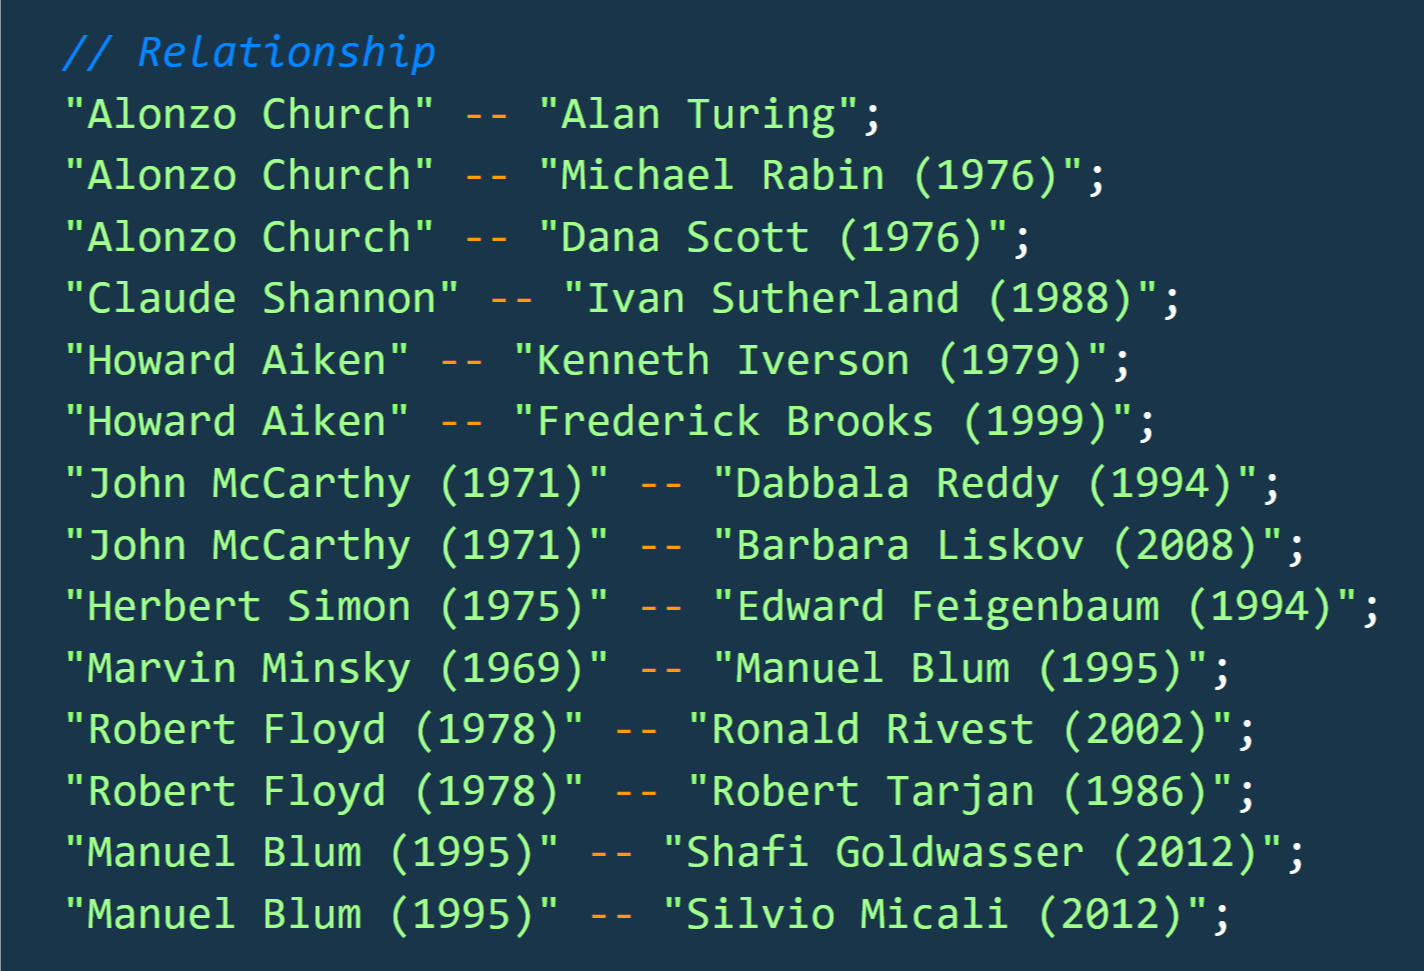
\includegraphics[scale = 0.63]{relbasic.png}
    \end{center}
    \end{frame}
    
\begin{frame}{GraphViz}

    \begin{columns}
        \begin{column}{0.5\textwidth}
           \begin{itemize}
            \item Command Line tool for drawing graphs
            \item Has two main models:
            \begin{itemize}
                \item Hirarchical graph structuring
                \item Spring/Force based structuring \pause
            \end{itemize}
            \vspace{0.5cm}
            \item Provides four main tools: 
            \begin{itemize}
                \item dot
                \item neato
                \item lefty 
                \item dotty \pause
            \end{itemize}
        \end{itemize}
        \end{column}
        \begin{column}{0.5\textwidth}  %%<--- here
            \begin{center}
             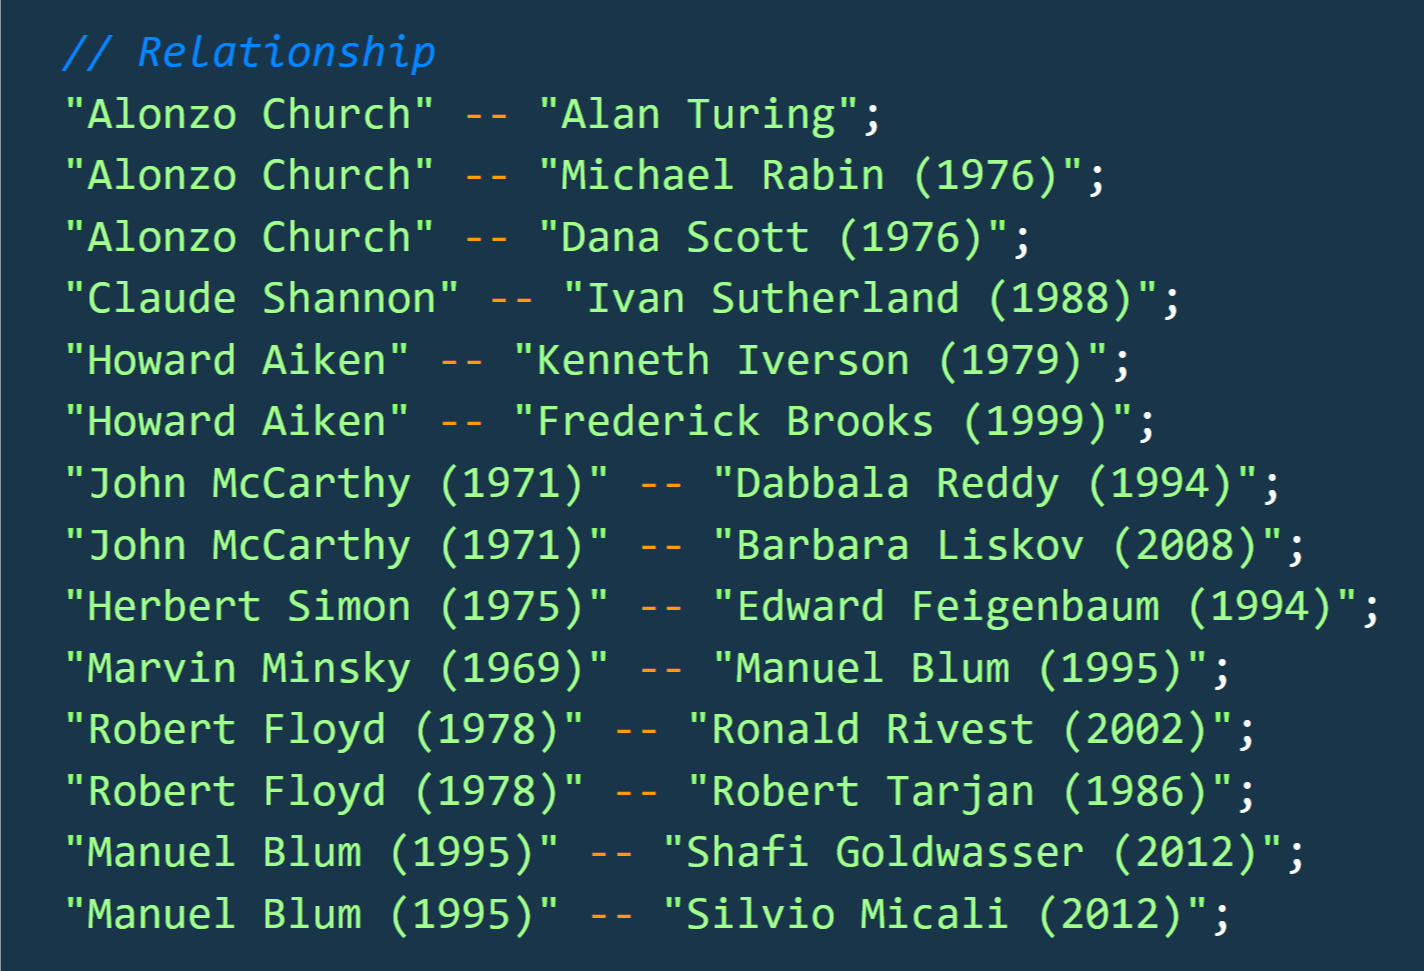
\includegraphics[width=1\textwidth]{relbasic.png}
             \end{center}
        \end{column}
    \end{columns}
\end{frame}

\begin{frame}{First Graph}
    \begin{center}
        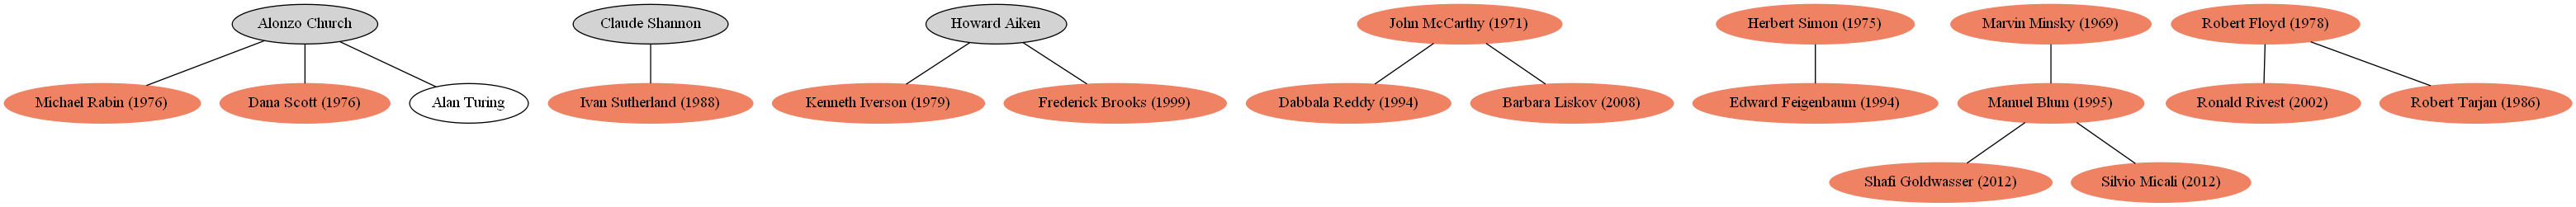
\includegraphics[scale = 0.14]{dotrel1.png}
        \pause
    \end{center}
    \begin{center}
        \vspace{1.0cm}
        Too disconnected...
    \end{center}
\end{frame}

\begin{frame}{First Hypothesis}
    \pause
    \begin{center}
        Graph should be more connected if I add the other relationships available in the book draft
        \pause

        \vspace{1.0cm}
        \begin{itemize}
            \item Co-authors
            \item Colleagues
            \item Prof-Student
            \item Necrologies/misc.
        \end{itemize}
    \end{center}
\end{frame}

\begin{frame}{Second Graph}
    \begin{center}
        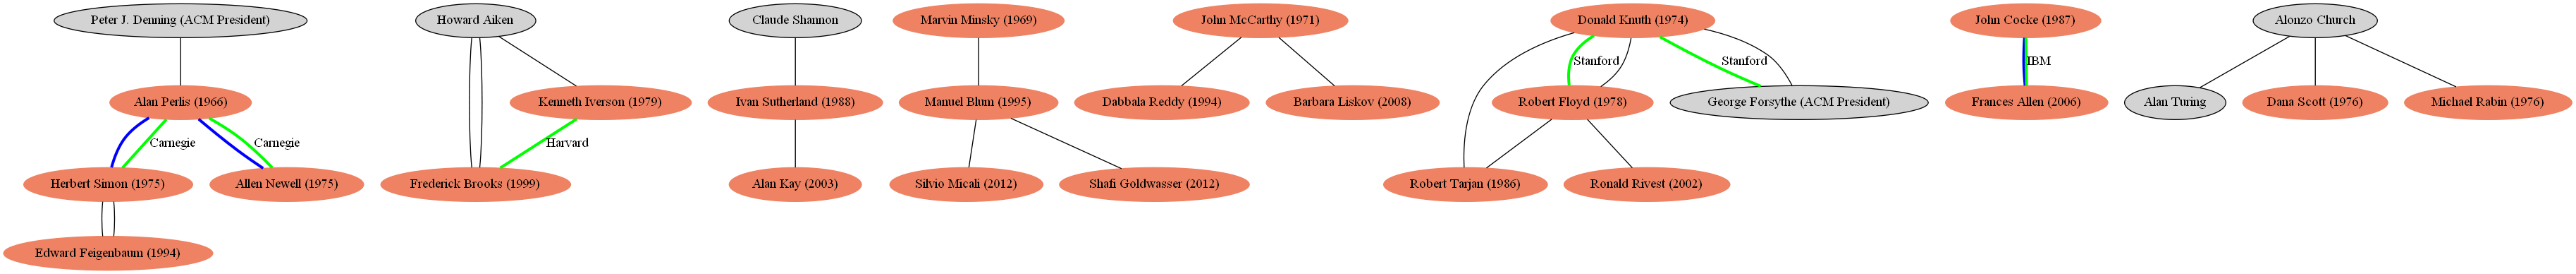
\includegraphics[scale = 0.12]{dotrel3.png}
    \end{center}
\end{frame}

\begin{frame}{First Graph}
    \begin{center}
        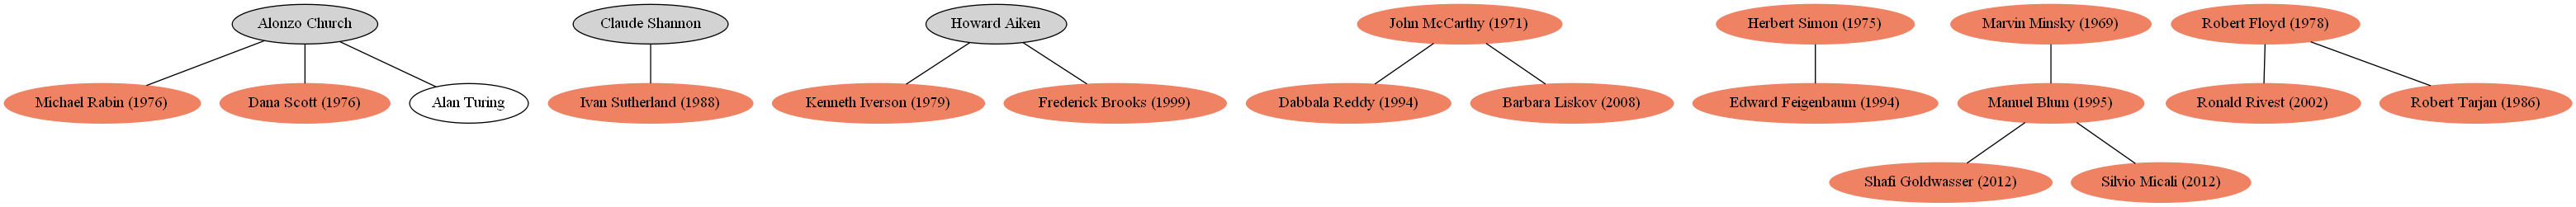
\includegraphics[scale = 0.14]{dotrel1.png}
    \end{center}
\end{frame}

\begin{frame}{Second Graph}
    \begin{center}
        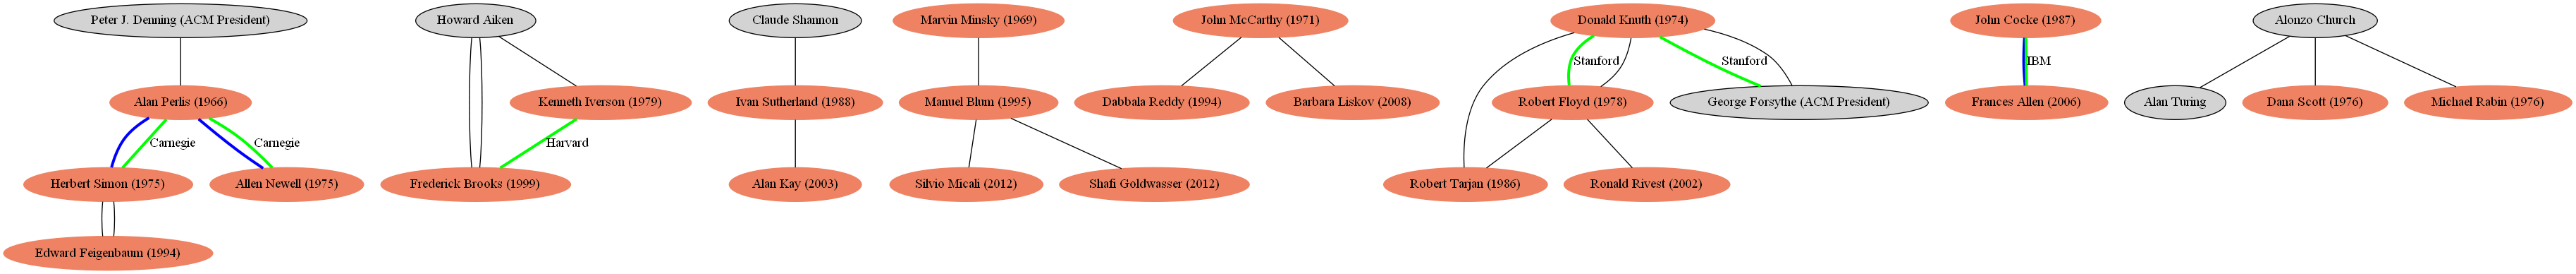
\includegraphics[scale = 0.12]{dotrel3.png}
        \pause
    \end{center}
    \begin{center}
        \vspace{1.0cm}
        Graph should be more connected if I add the other relationships available in the book draft
    \end{center}
\end{frame}

\begin{frame}{Third Graph}

    \begin{center}
        Need more data\\ \pause
        \vspace{1.0cm}
        Hypothysis 2: If I get the PhD supervisor(s) of every Turing awardee then I should get a more well constructed graph
    \end{center}

\end{frame}

\begin{frame}{Getting the Data}
    \pause
    \begin{center}
        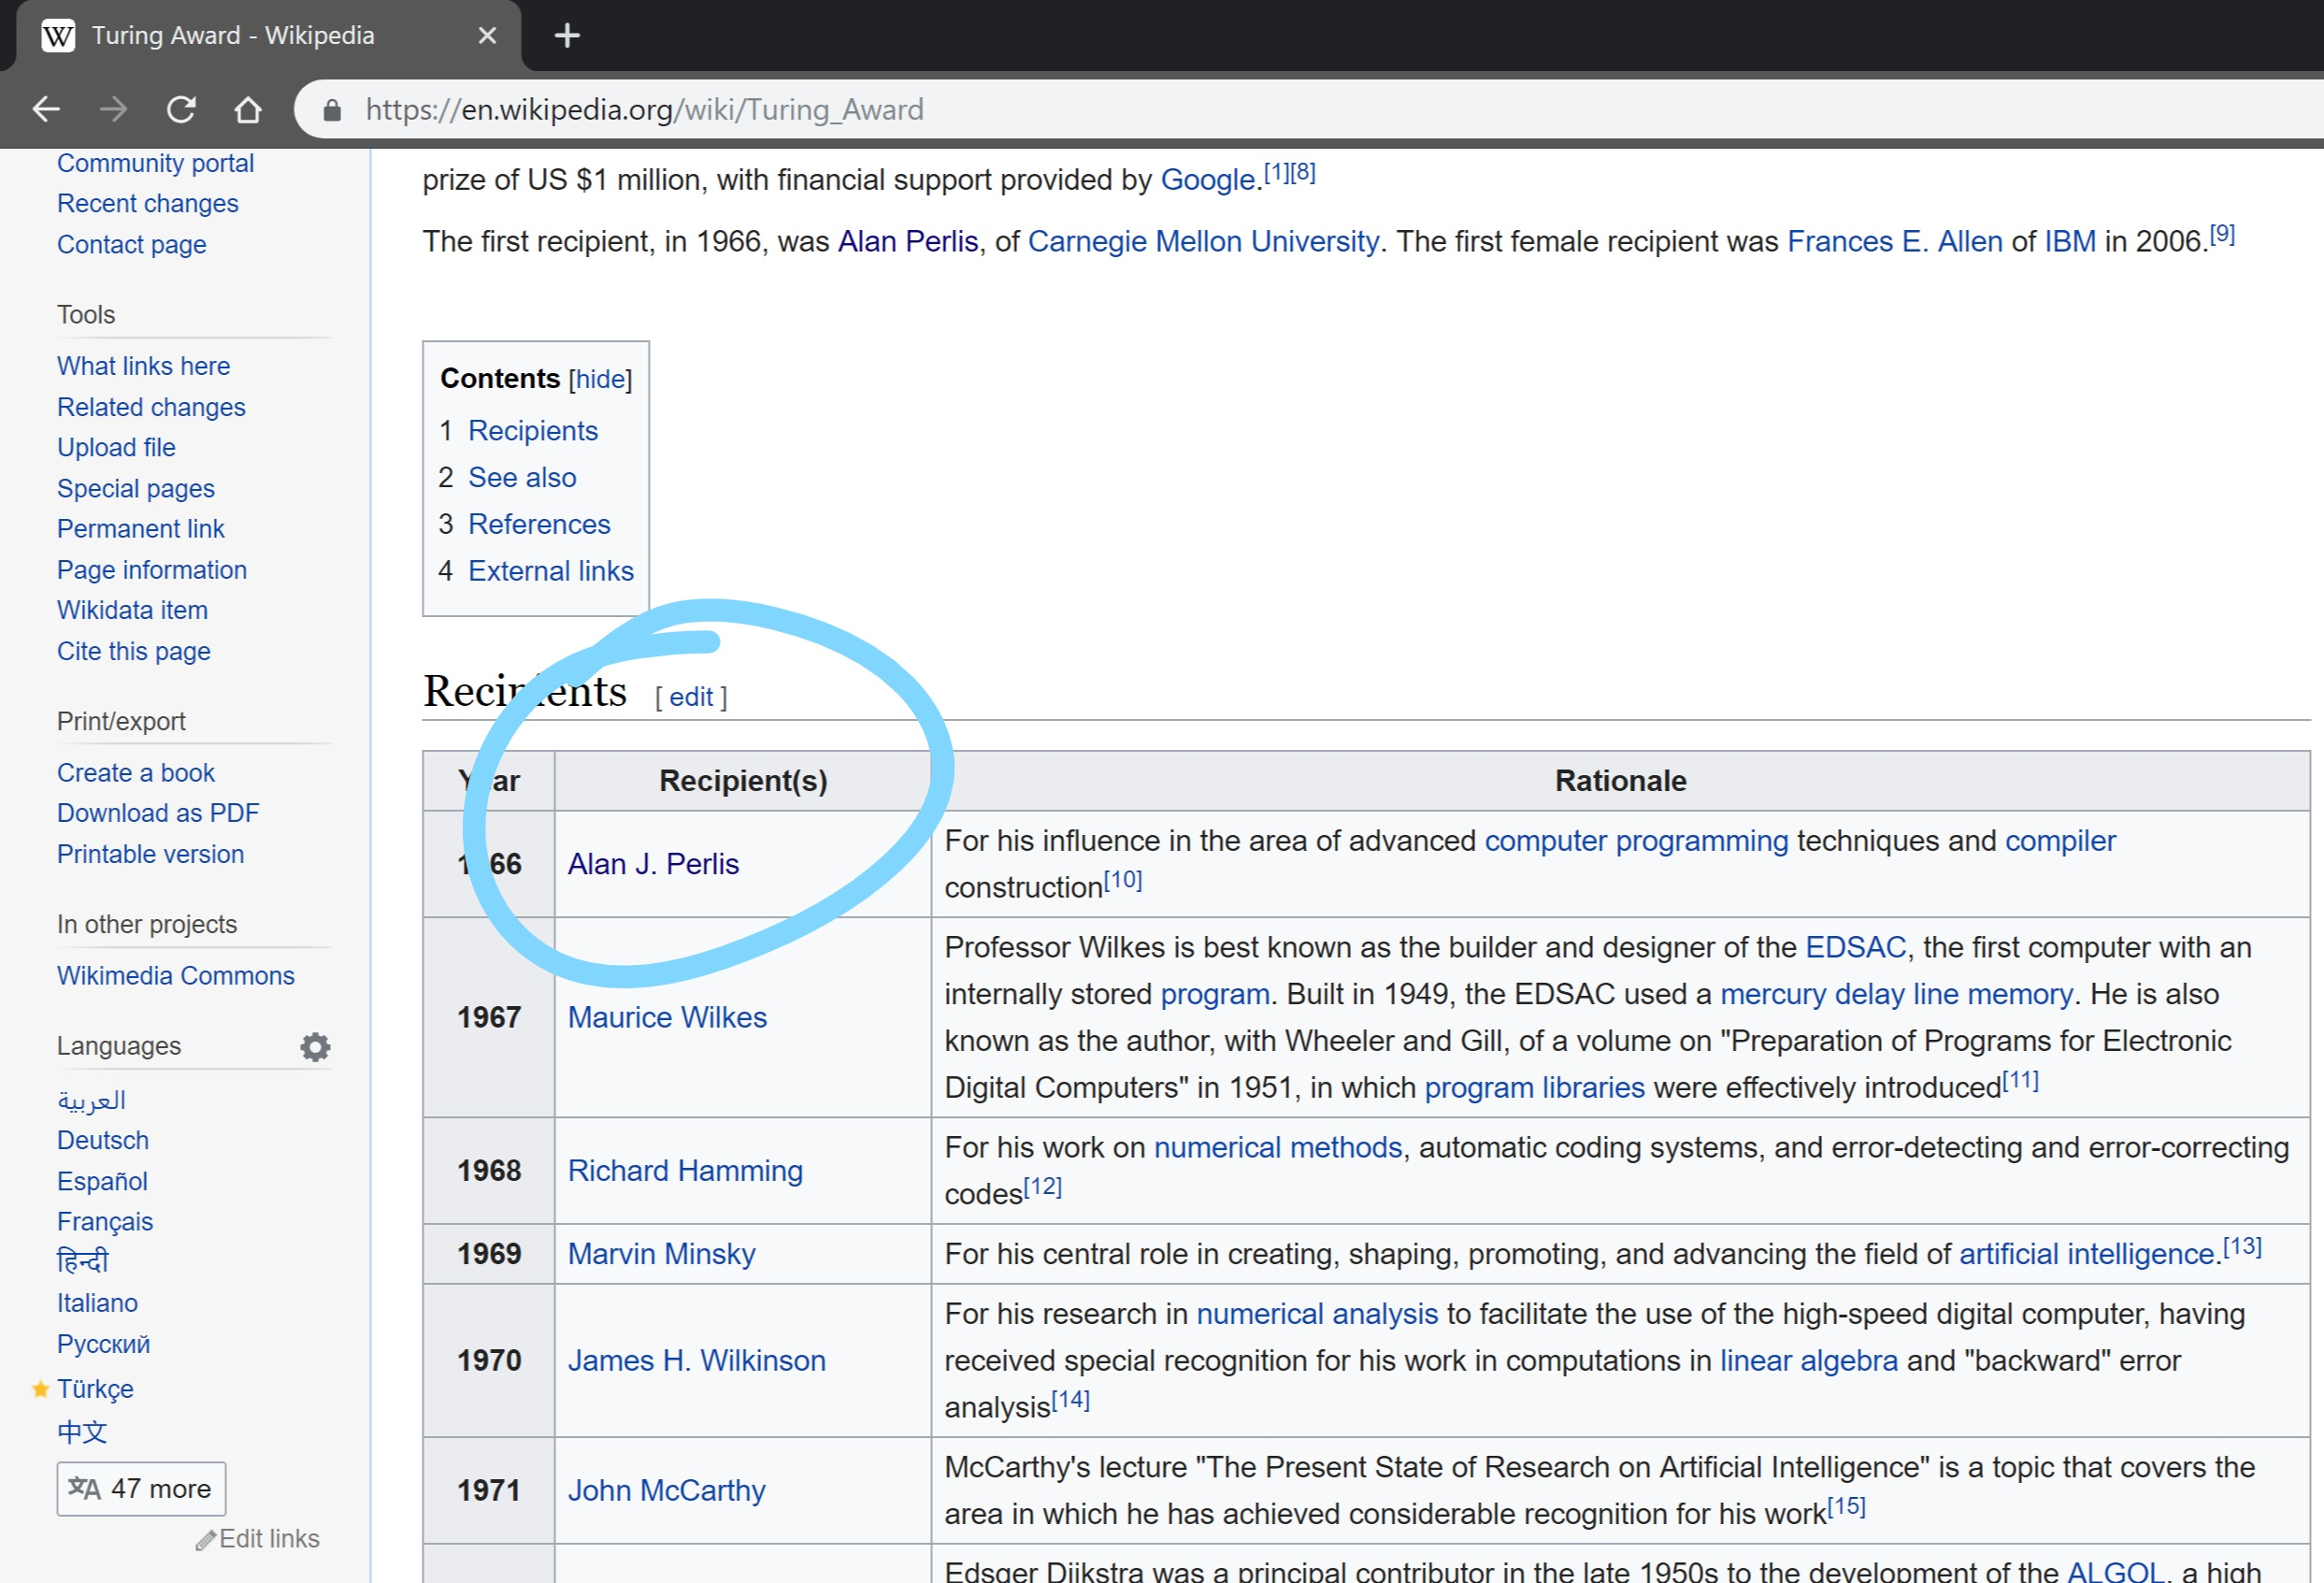
\includegraphics[scale=0.13]{wiki.jpg}
    \end{center}
\end{frame}

\begin{frame}{Getting the Data}
    \begin{center}
        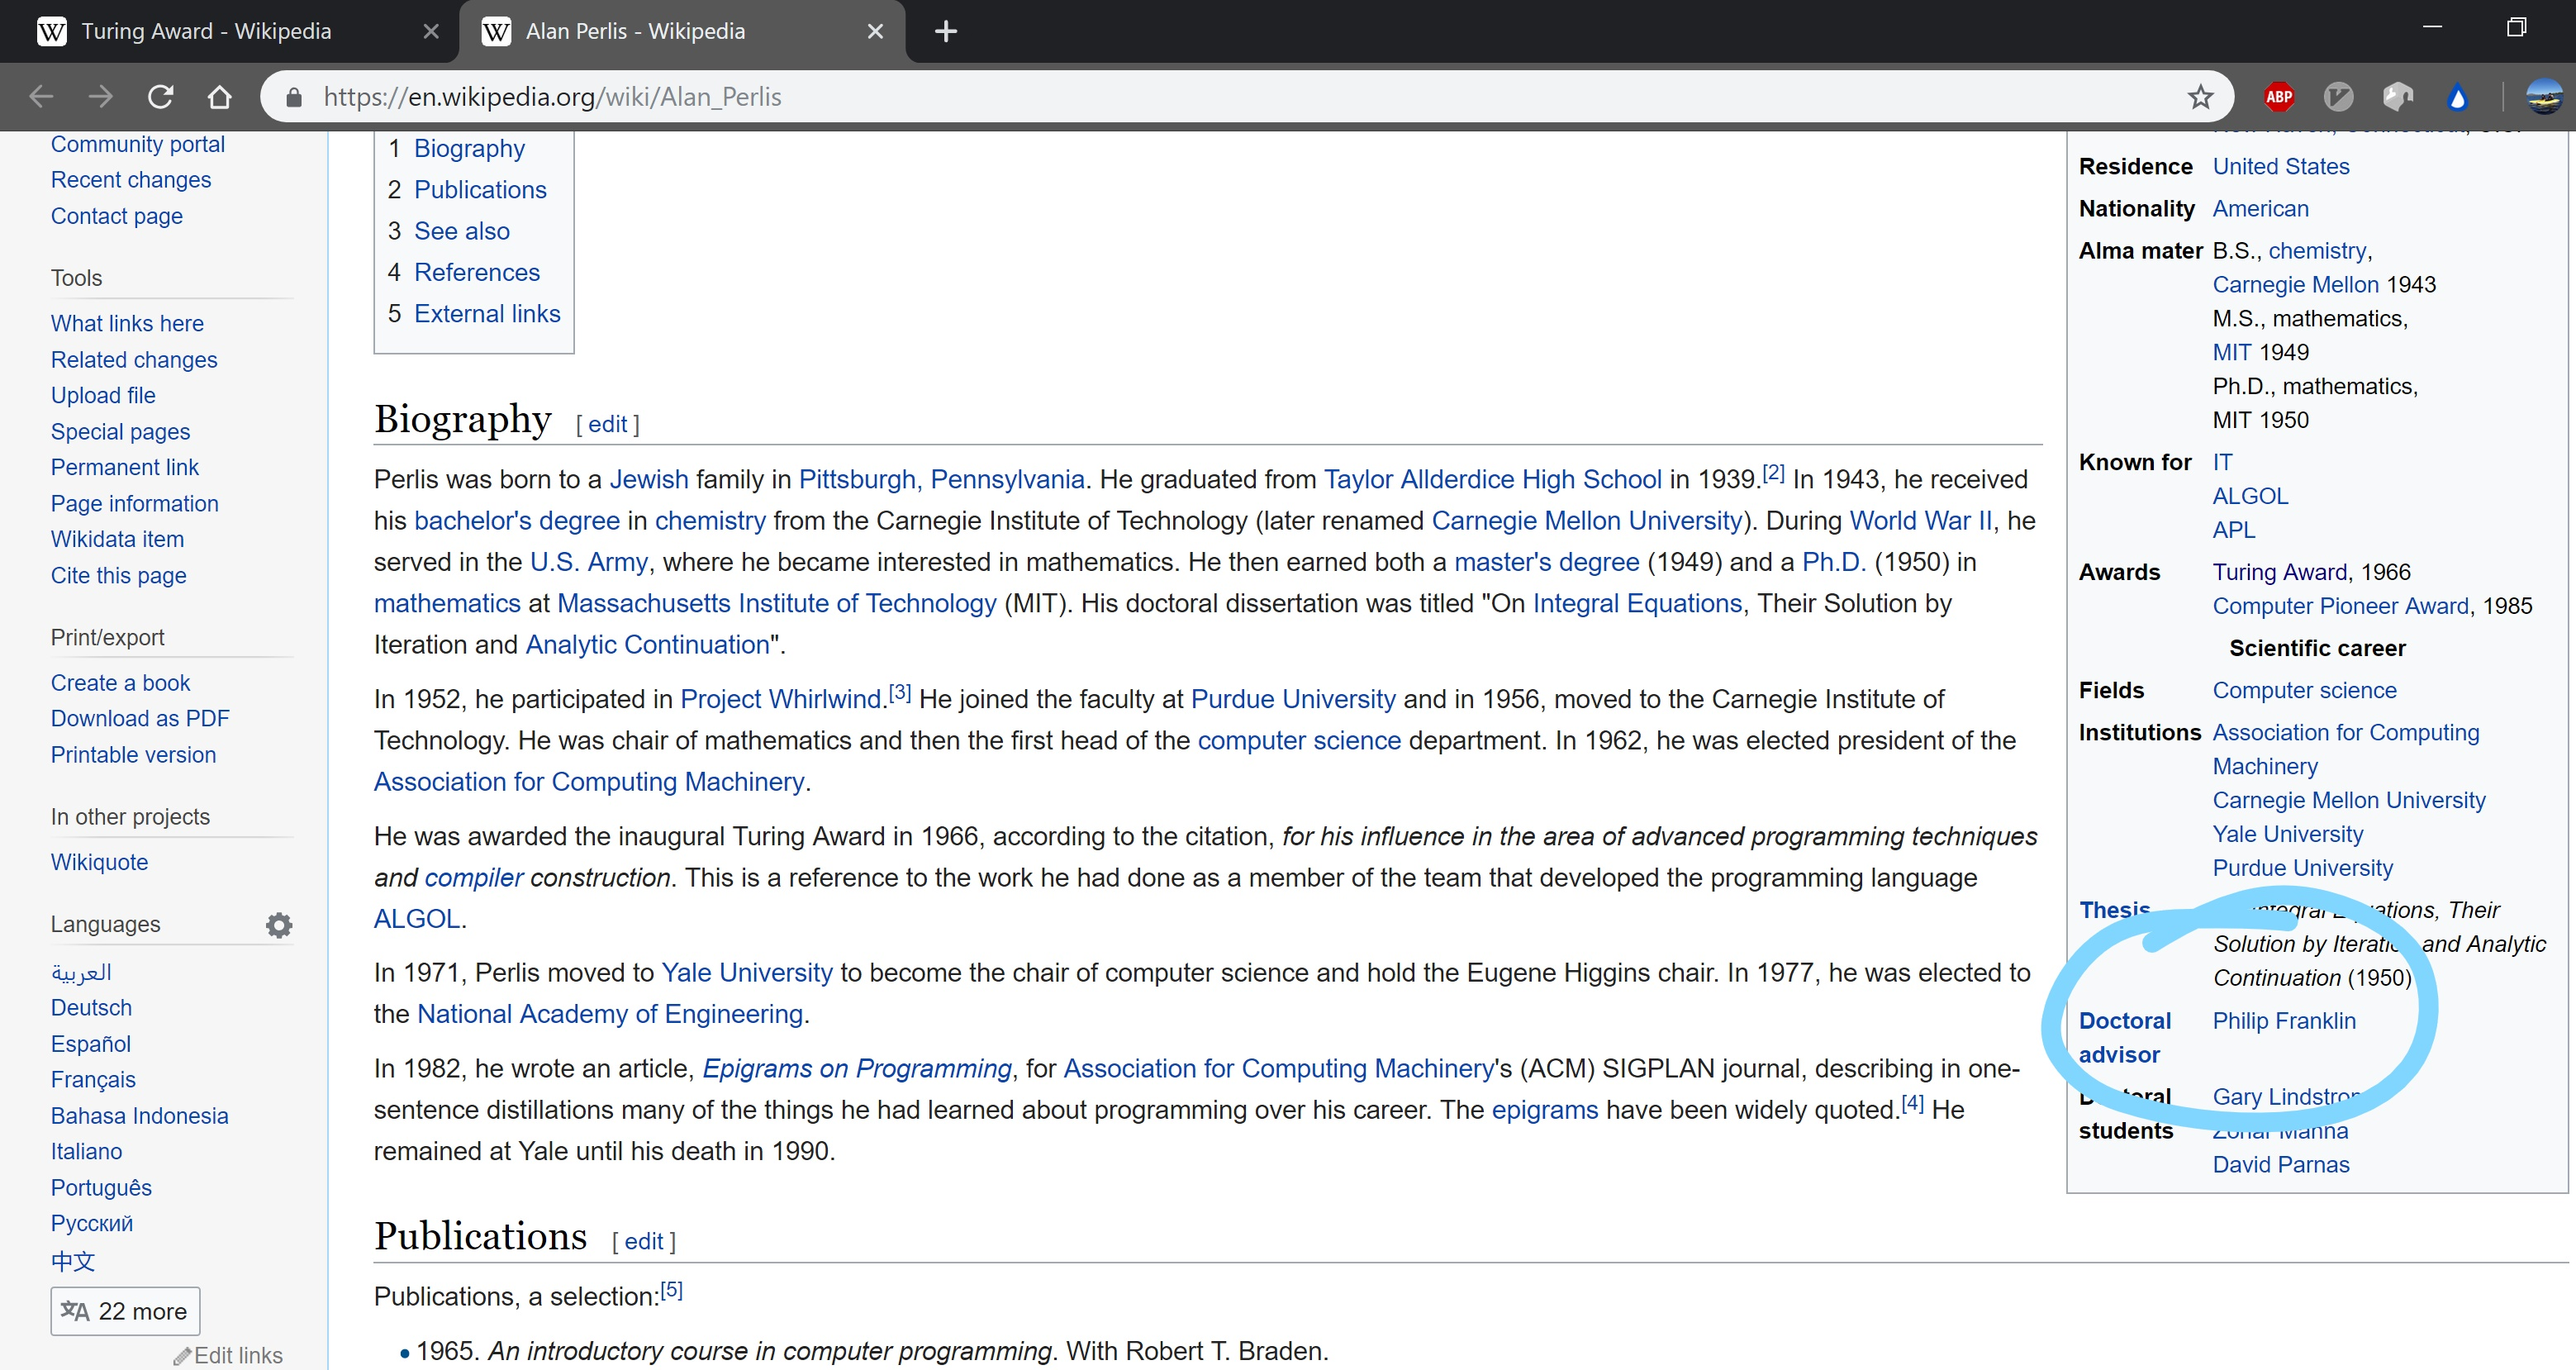
\includegraphics[scale=0.13]{wiki2.jpg}
    \end{center}
\end{frame}

\begin{frame}{Third Graph}
    \begin{center}
        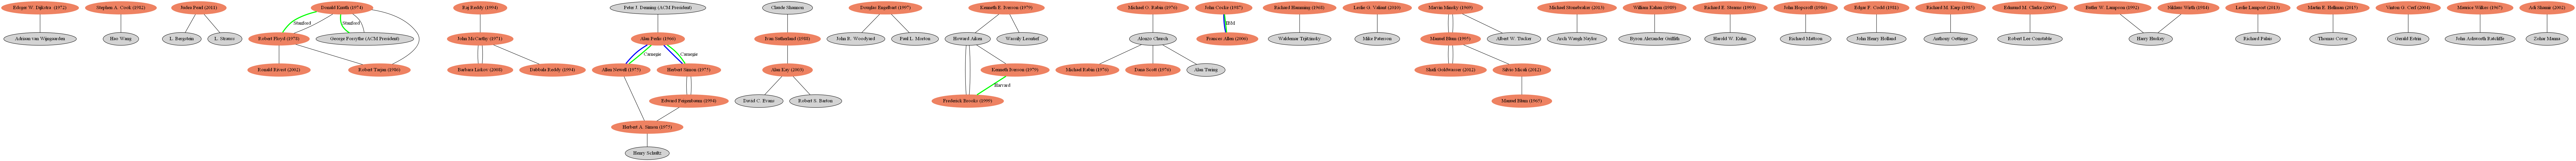
\includegraphics[scale = 0.045]{dotrel4.png}
    \end{center}
\end{frame}

\begin{frame}{Third Graph}
    \vspace{-0.5cm}
    \begin{center}
        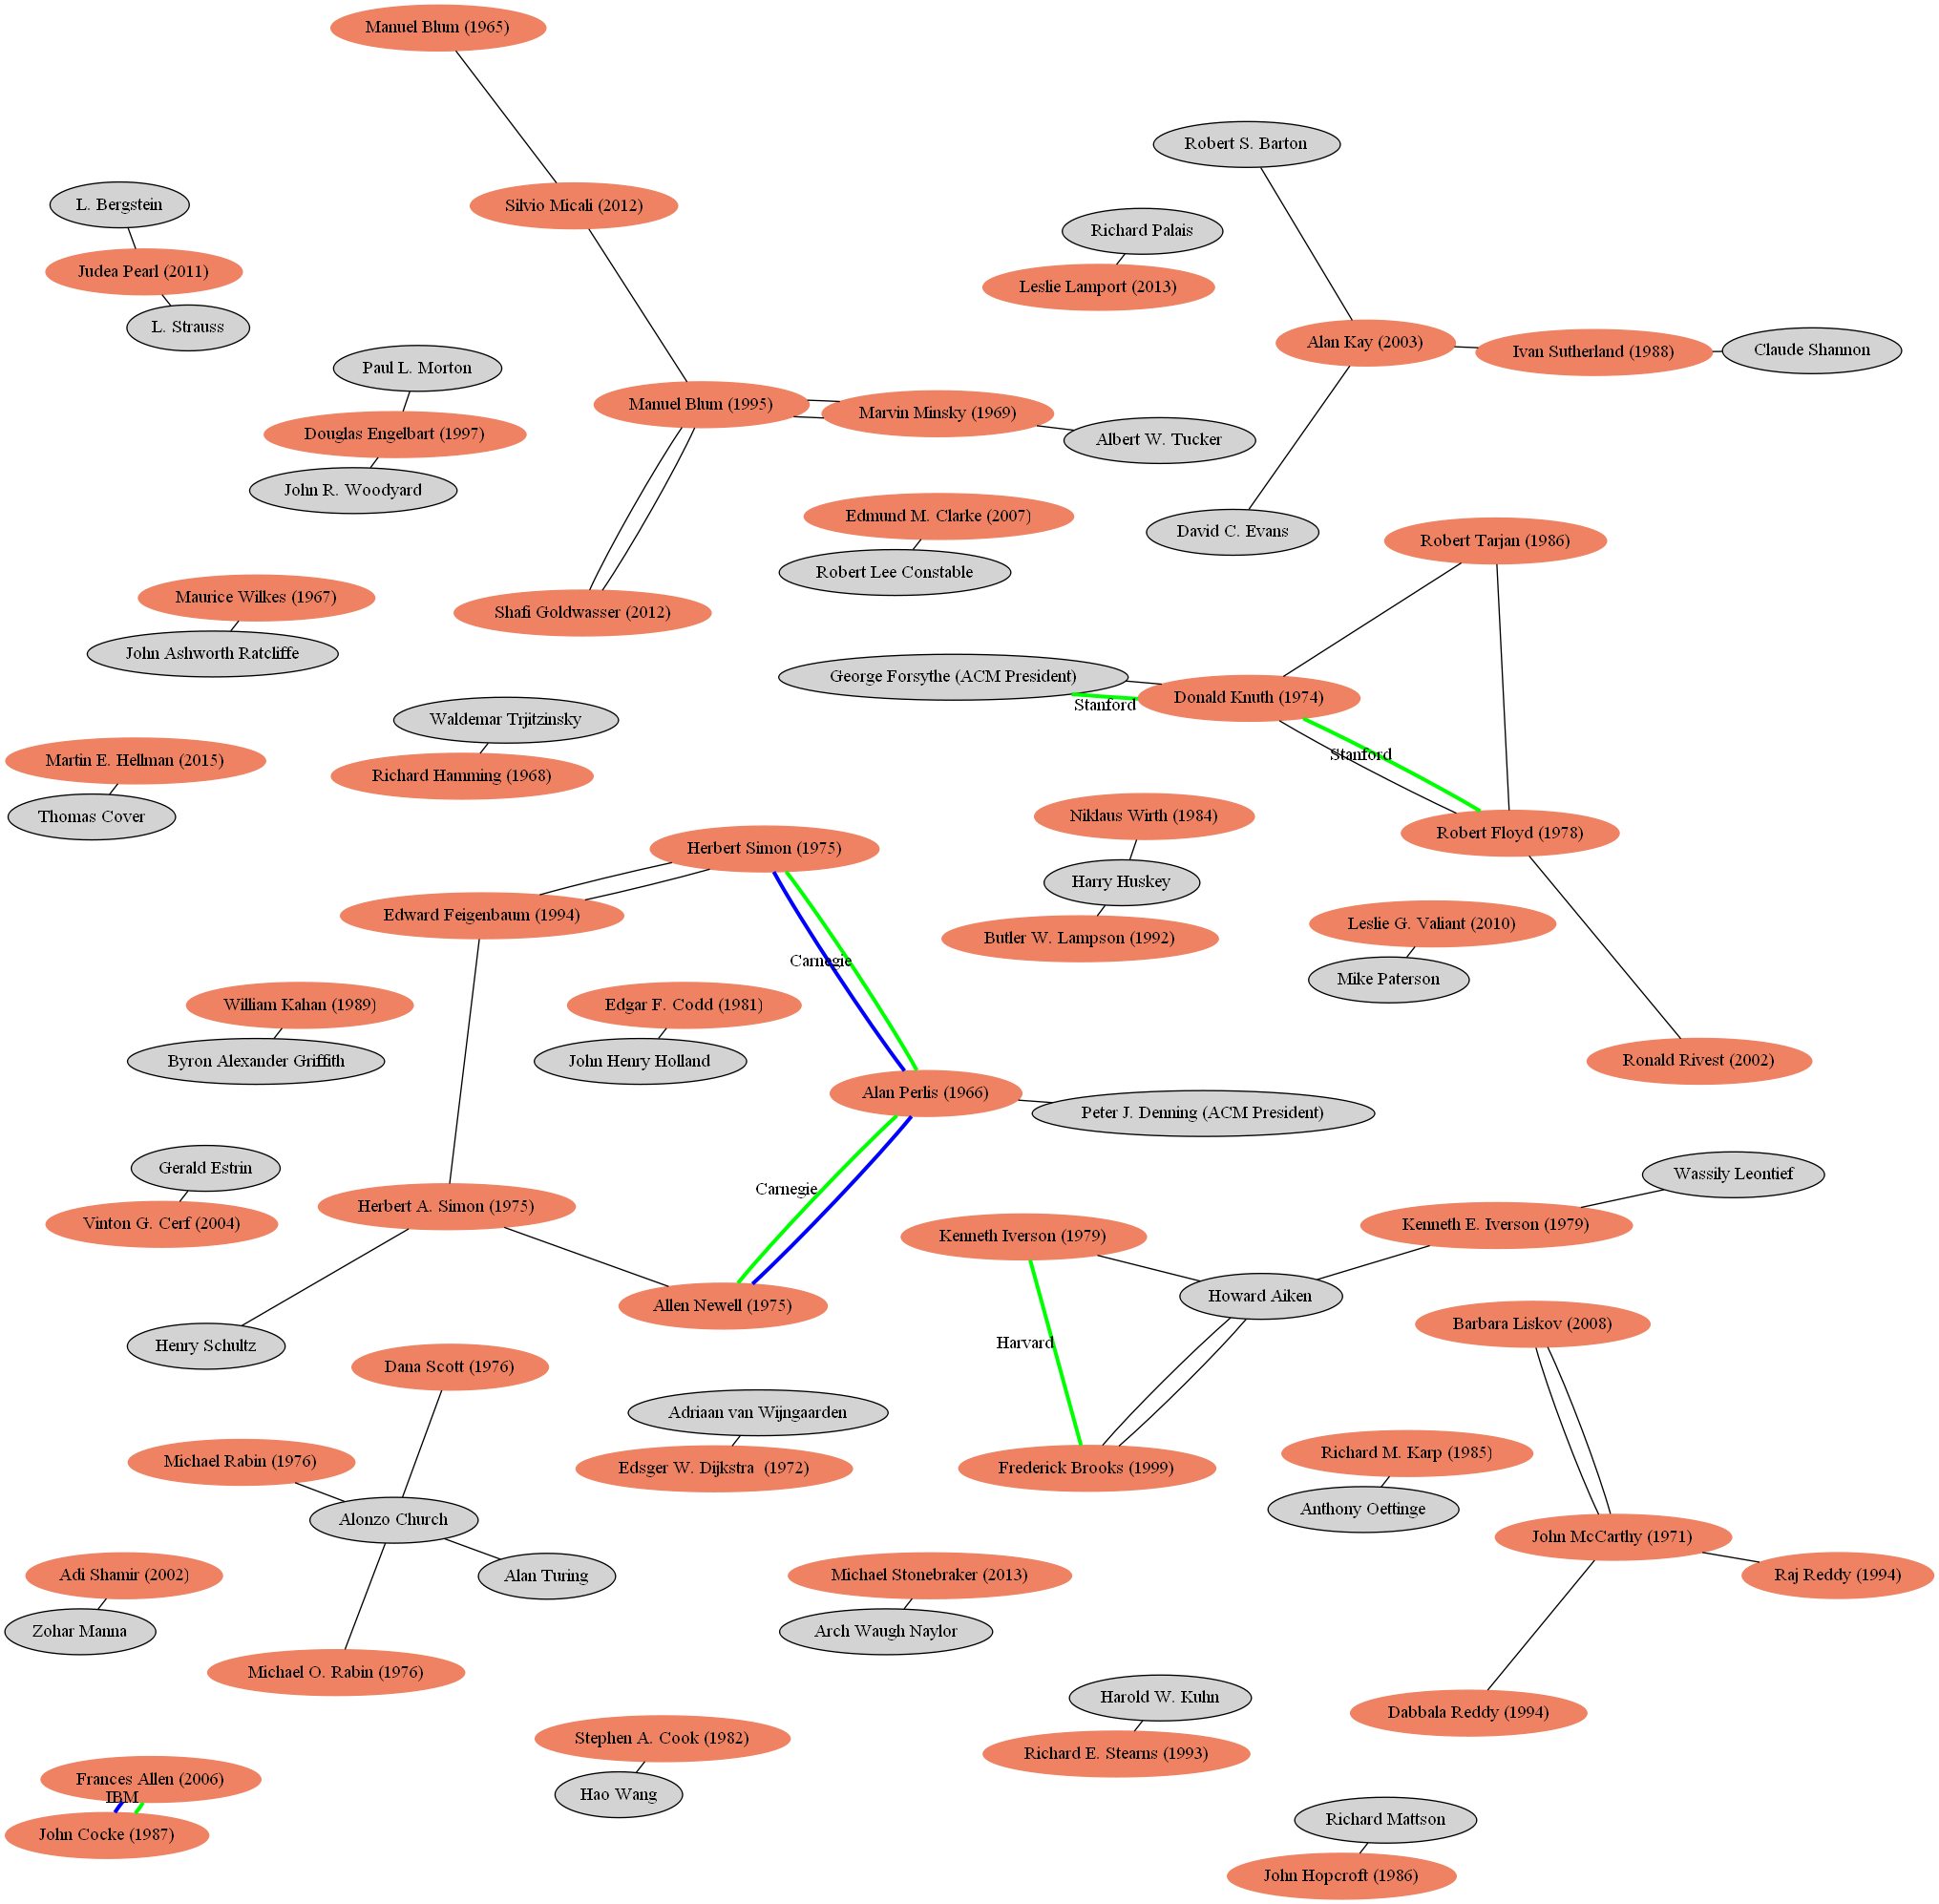
\includegraphics[scale = 0.11]{neatorel4.png}
    \end{center}
\end{frame}

\begin{frame}{Fourth Graph}
    \begin{center}
        What is a way that guarantees connection?
    \end{center}
\end{frame}

\begin{frame}{Fourth Graph}
    \begin{center}
        What is a good way that guarantees connection?
    \end{center}
    \pause
    \begin{itemize}
        \item Field of research \pause
        \begin{itemize}
            \item Mathematics
            \item Compilers
            \item Web
            \item Architecture
            \item Algorithms
            \item Operating System
            \item Distributed Computing
            \item Mathematics
            \item Database
            \item Artificial Intelligence
            \item Automata
        \end{itemize}
    \end{itemize}
\end{frame}

\begin{frame}{Fourth Graph}
    \vspace{-0.25cm}
        \begin{center}
            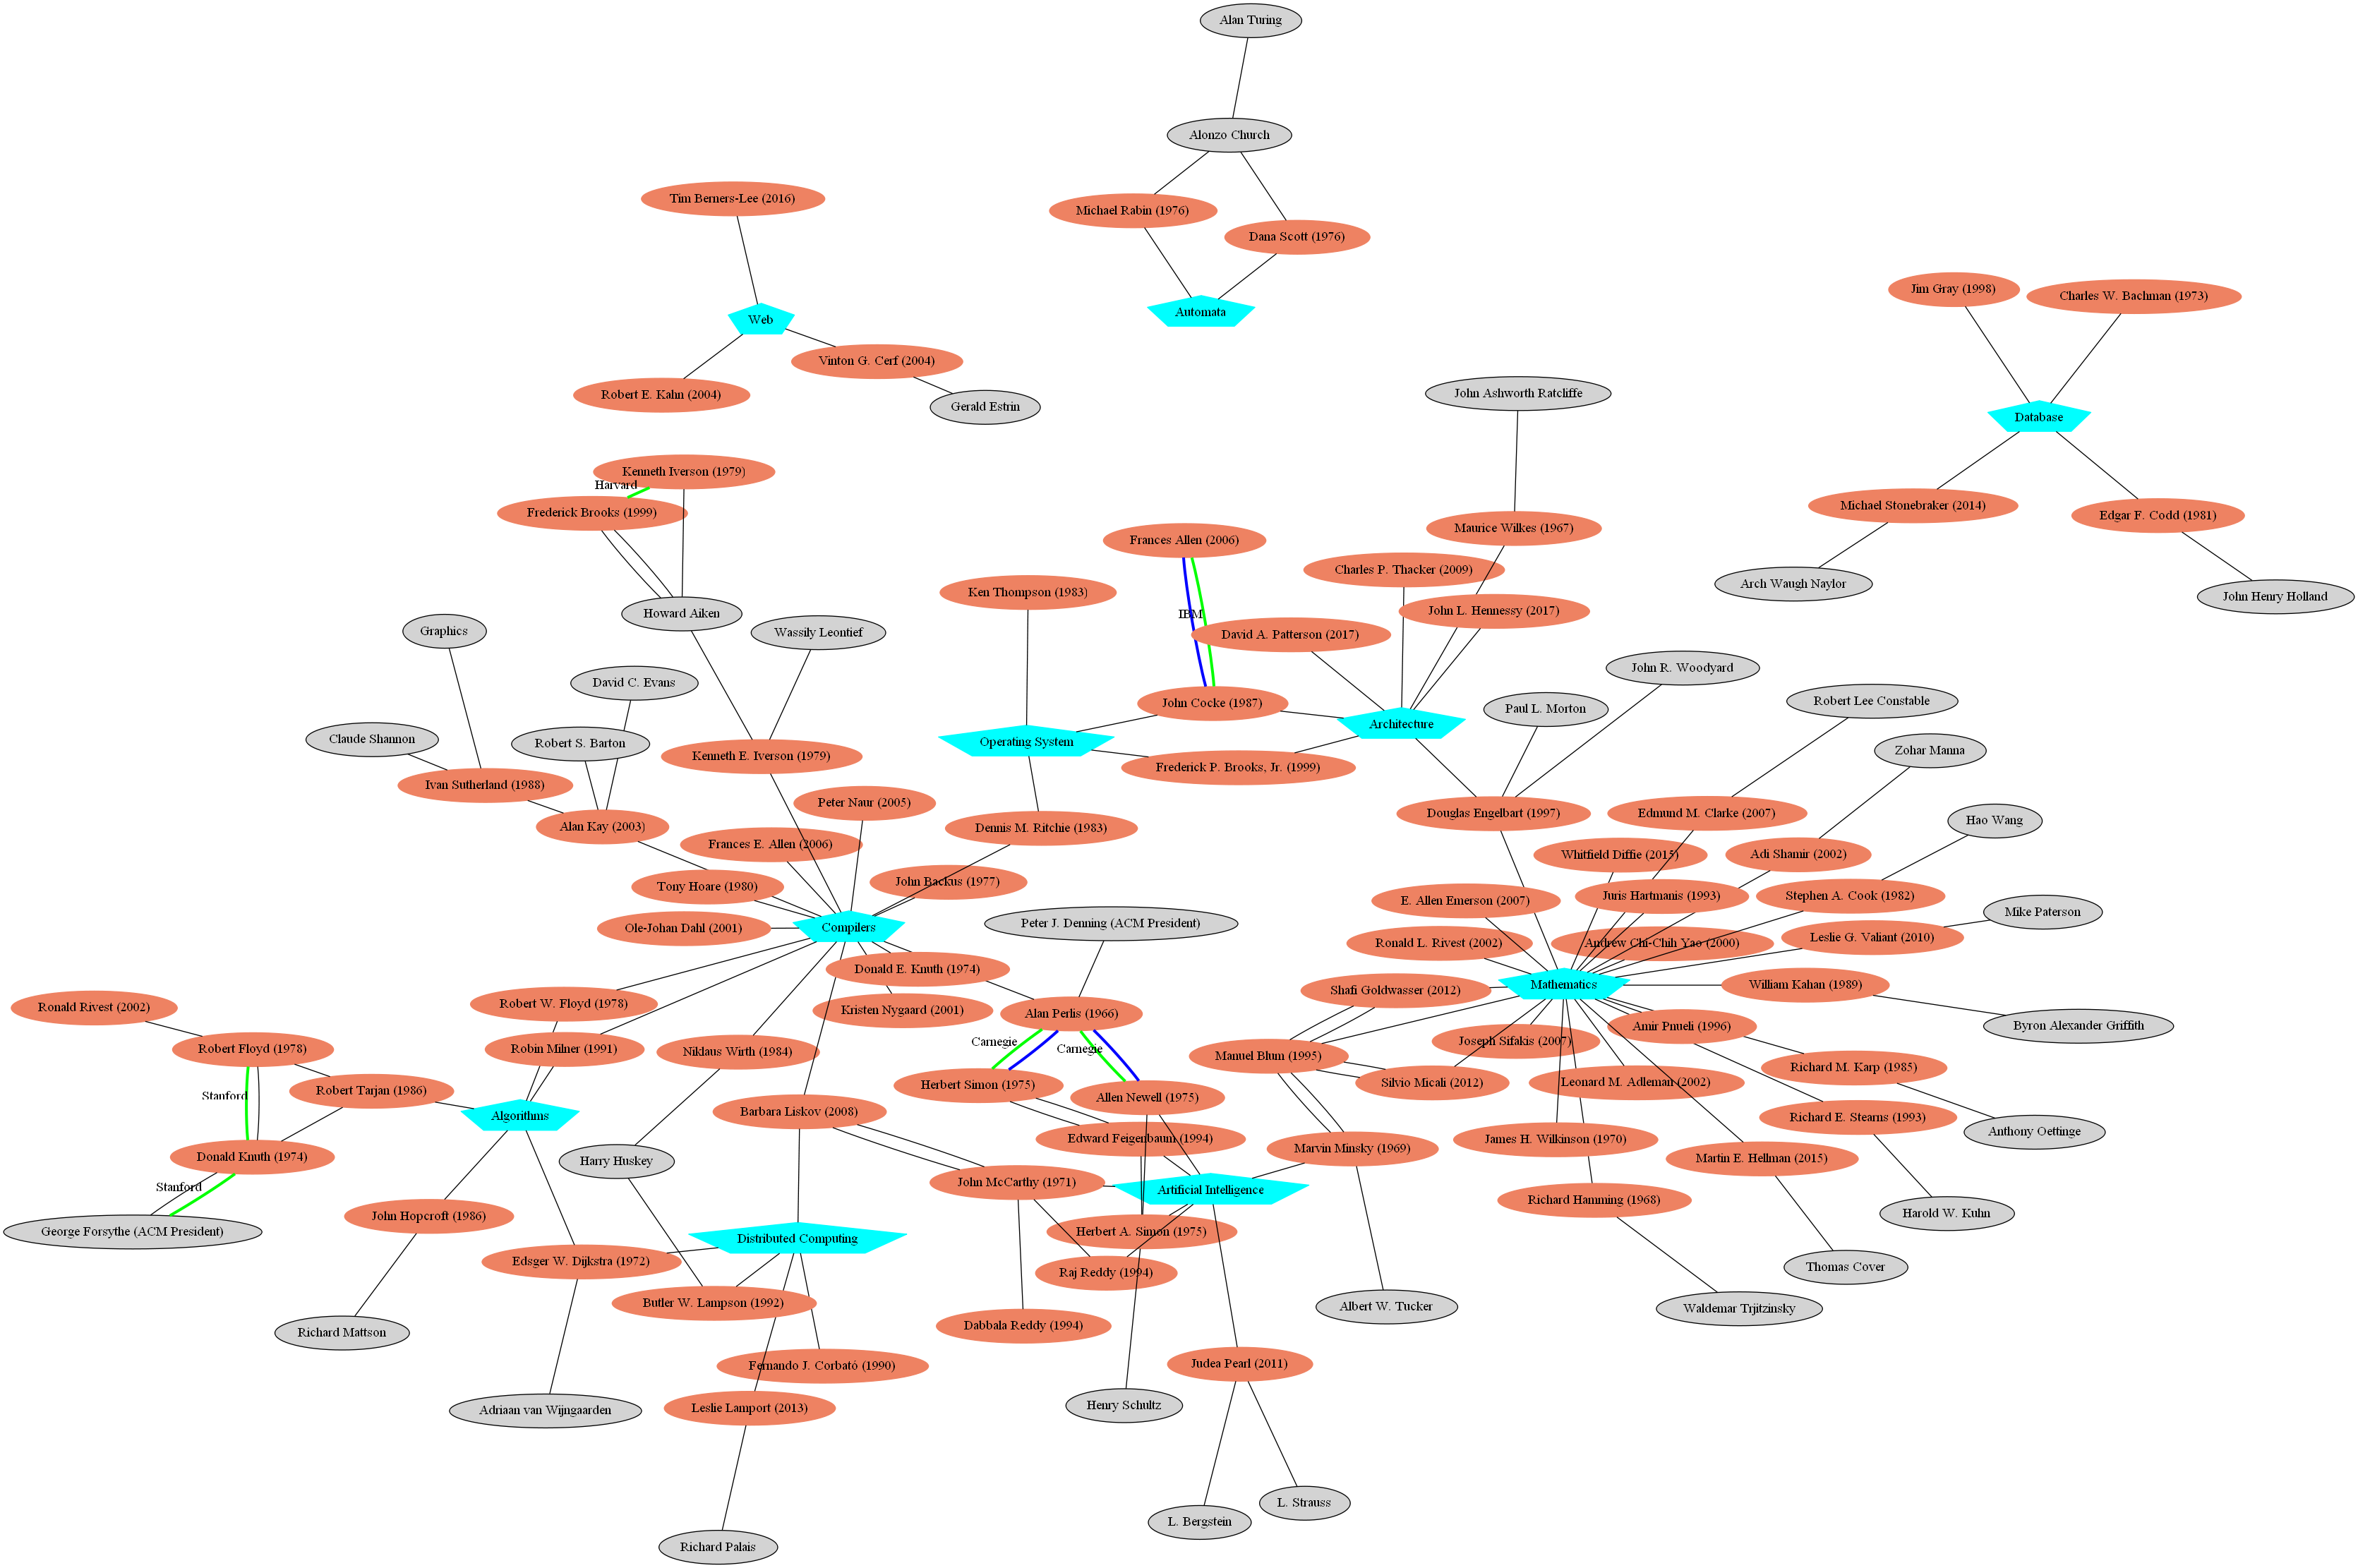
\includegraphics[scale=0.1]{neatorel5.png}
        \end{center}
\end{frame}

\begin{frame}{Fourth Graph}
        \begin{center}
            
\includegraphics[scale=0.033]{dotrel5.png}
        \end{center}
\end{frame}

\end{document}